\begin{figure}[H]
    \centering
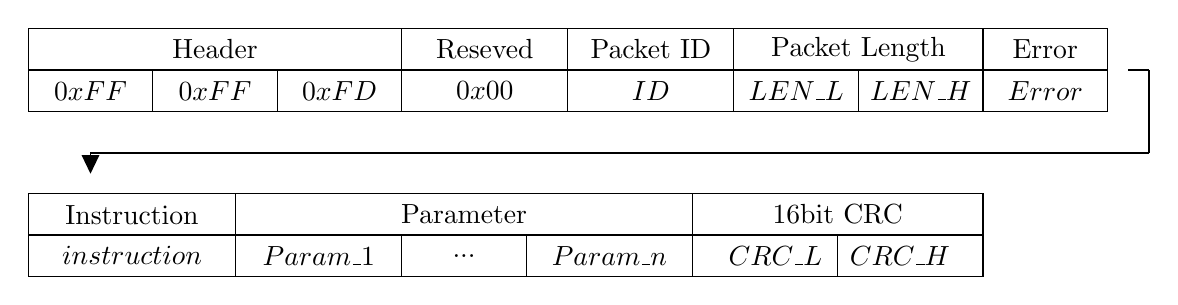
\begin{tikzpicture}[x=0.75pt,y=0.75pt,yscale=-1,xscale=1]
%uncomment if require: \path (0,158.99999237060547); %set diagram left start at 0, and has height of 158.99999237060547

%Shape: Rectangle [id:dp8698497909833363] 
\draw   (10,30) -- (70,30) -- (70,50) -- (10,50) -- cycle ;
%Shape: Rectangle [id:dp6485581117247297] 
\draw   (70,30) -- (130,30) -- (130,50) -- (70,50) -- cycle ;
%Shape: Rectangle [id:dp6658546174120246] 
\draw   (130,30) -- (190,30) -- (190,50) -- (130,50) -- cycle ;
%Shape: Rectangle [id:dp6752872057996913] 
\draw   (190,30) -- (270,30) -- (270,50) -- (190,50) -- cycle ;
%Shape: Rectangle [id:dp5014813538264575] 
\draw   (350,30) -- (410,30) -- (410,50) -- (350,50) -- cycle ;
%Shape: Rectangle [id:dp7457170593383808] 
\draw   (410,30) -- (470,30) -- (470,50) -- (410,50) -- cycle ;
%Shape: Rectangle [id:dp5054173748421811] 
\draw   (270,30) -- (350,30) -- (350,50) -- (270,50) -- cycle ;
%Shape: Rectangle [id:dp1263298518018401] 
\draw   (10,109.5) -- (110,109.5) -- (110,129.5) -- (10,129.5) -- cycle ;
%Shape: Rectangle [id:dp6896214683381987] 
\draw   (110,109.5) -- (190,109.5) -- (190,129.5) -- (110,129.5) -- cycle ;
%Shape: Rectangle [id:dp8350012688131694] 
\draw   (330,89.5) -- (470,89.5) -- (470,109.5) -- (330,109.5) -- cycle ;
%Shape: Rectangle [id:dp8375426281198146] 
\draw   (190,109.5) -- (250,109.5) -- (250,129.5) -- (190,129.5) -- cycle ;
%Shape: Rectangle [id:dp6586789788358929] 
\draw   (330,109.5) -- (400,109.5) -- (400,129.5) -- (330,129.5) -- cycle ;
%Shape: Rectangle [id:dp14973963332658702] 
\draw   (10,10) -- (190,10) -- (190,30) -- (10,30) -- cycle ;
%Shape: Rectangle [id:dp30939097077443956] 
\draw   (190,10) -- (270,10) -- (270,30) -- (190,30) -- cycle ;
%Shape: Rectangle [id:dp20452238276938295] 
\draw   (350,10) -- (470,10) -- (470,30) -- (350,30) -- cycle ;
%Shape: Rectangle [id:dp08631851455147288] 
\draw   (270,10) -- (350,10) -- (350,30) -- (270,30) -- cycle ;
%Shape: Rectangle [id:dp351731230245929] 
\draw   (10,89.5) -- (110,89.5) -- (110,109.5) -- (10,109.5) -- cycle ;
%Shape: Rectangle [id:dp46139057893485447] 
\draw   (250,109.5) -- (330,109.5) -- (330,129.5) -- (250,129.5) -- cycle ;
%Shape: Rectangle [id:dp42456037527605517] 
\draw   (110,89.5) -- (330,89.5) -- (330,109.5) -- (110,109.5) -- cycle ;
%Shape: Rectangle [id:dp5173327089860826] 
\draw   (400,109.5) -- (470,109.5) -- (470,129.5) -- (400,129.5) -- cycle ;
%Straight Lines [id:da19477344689590792] 
\draw    (550,70) -- (40,70) ;


%Straight Lines [id:da31415506805713345] 
\draw    (40,70) -- (40,78) ;
\draw [shift={(40,80)}, rotate = 270] [fill={rgb, 255:red, 0; green, 0; blue, 0 }  ][line width=0.75]  [draw opacity=0] (8.93,-4.29) -- (0,0) -- (8.93,4.29) -- cycle    ;

%Shape: Rectangle [id:dp13994941859002452] 
\draw   (470,10) -- (530,10) -- (530,30) -- (470,30) -- cycle ;
%Shape: Rectangle [id:dp04644653628071138] 
\draw   (470,30) -- (530,30) -- (530,50) -- (470,50) -- cycle ;
%Straight Lines [id:da3764266198993005] 
\draw    (550,70) -- (550,30) ;


%Straight Lines [id:da06827427289797416] 
\draw    (540,30) -- (550,30) ;



% Text Node
\draw (40,40) node   {$0xFF$};
% Text Node
\draw (100,40) node   {$0xFF$};
% Text Node
\draw (160,40) node   {$0xFD$};
% Text Node
\draw (100,20) node  [align=left] {Header};
% Text Node
\draw (230,20) node  [align=left] {Reseved};
% Text Node
\draw (230,40) node   {$0x00$};
% Text Node
\draw (310,40) node   {$ID$};
% Text Node
\draw (310,20) node  [align=left] {Packet ID};
% Text Node
\draw (380,40) node   {$LEN\_L$};
% Text Node
\draw (440,40) node   {$LEN\_H$};
% Text Node
\draw (410,20) node  [align=left] {Packet Length};
% Text Node
\draw (60,119.5) node   {$instruction$};
% Text Node
\draw (60,100) node  [align=left] {Instruction};
% Text Node
\draw (150,119.5) node   {$Param\_1$};
% Text Node
\draw (220,119.5) node   {$...$};
% Text Node
\draw (290,119.5) node   {$Param\_n$};
% Text Node
\draw (220,99.5) node  [align=left] {Parameter};
% Text Node
\draw (370,119.5) node   {$CRC\_L$};
% Text Node
\draw (430,119.5) node   {$CRC\_H$};
% Text Node
\draw (400,99.5) node  [align=left] {16bit CRC};
% Text Node
\draw (500,20) node  [align=left] {Error};
% Text Node
\draw (500,40) node   {$Error$};


\end{tikzpicture}

    \caption{Structure of the status packet\cite{PIDmxx}}
    \label{fig:StatusStruct}
\end{figure}